\documentclass[xcolor={dvipsnames,table},aspectratio=169]{beamer}
\usepackage[utf8]{inputenc}
\usepackage[T1]{fontenc}
\usepackage[brazil]{babel}
\usepackage{graphics,amssymb,amsfonts,amsmath}
\usepackage{tikz}
\usepackage{enumerate,hyperref}
\usepackage{palatino}
\usepackage{ragged2e}
\usepackage{minted}
\usepackage{booktabs}
\usepackage{verbatim}
\usepackage[export]{adjustbox}
\usepackage{tikz}                   
\usepackage{xcolor}
\usepackage{textcomp} % para usar \textdegree
\usetikzlibrary{shadows}
\usetheme{AnnArbor}
\usecolortheme{orchid}
\usefonttheme[onlymath]{serif}

\newminted{java}{bgcolor=cyan!10}

\newcolumntype{C}[1]{>{\centering\let\newline\\\arraybackslash\hspace{0pt}}m{#1}}

\AtBeginSection[]{
  \begin{frame}
  \vfill
  \centering
  \begin{beamercolorbox}[sep=8pt,center,shadow=true,rounded=true]{title}
    \usebeamerfont{title}\insertsectionhead\par%
  \end{beamercolorbox}
  \vfill
  \end{frame}
}

\title[\sc{Laços}]{Laços}
\author[Roland Teodorowitsch]{Roland Teodorowitsch}
\institute[FPROG - EP - PUCRS]{Fundamentos de Programação - Escola Politécnica - PUCRS}
\date{4 de maio de 2023}

\begin{document}
\justifying

%-------------------------------------------------------
\begin{frame}
	\titlepage
\end{frame}

%=======================================================
\section{Introdução}

%-------------------------------------------------------
\begin{frame}\frametitle{Objetivos}
\begin{itemize}
	\item Implementar laços com \texttt{while}, \texttt{for} e \texttt{do}
	\item Acompanhar a execução de um programa manualmente
	\item Familiarizar-se com os algoritmos comuns com laços
	\item Entender laços aninhados
	\item Implementar programas que leem e processam conjuntos de dados
\end{itemize}
\end{frame}

%-------------------------------------------------------
\begin{frame}\frametitle{Conteúdos}
\begin{itemize}
	\item O Laço \texttt{while}
	\item Exercícios
	\item O Laço \texttt{for}
	\item O Laço \texttt{do}
	\item Sentinelas de Processamento
	\item Algoritmos Comuns com Laços
	\item Laços Aninhados
	\item Resumo
\end{itemize}
\end{frame}

%=======================================================
\section{O Laço \texttt{while}}

%-------------------------------------------------------
\begin{frame}[fragile]\frametitle{Laços}
\begin{itemize}
	\item Um laço serve para repetir a execução de trechos de um programa\\
	\item Laços executam instruções repetidamente enquanto uma condição for verdadeira\\
	\item Exemplos de aplicações com laços\\
	\begin{itemize}
		\item Executar um processamento específico sobre um conjunto predefinido de dados\\\emph{\tiny Leia o raio de 10 círculos e mostre a área e a circunferência de cada círculo.}\\
		\item Executar um processamento específico sobre um conjunto de dados cujo tamanho foi fornecido\\\emph{\tiny Leia quantos círculos serão processados, e a seguir leia o raio de cada círculo, calculando a sua área e circunferência.}\\
		\item Executar um processamento específico sobre um conjunto indeterminado de dados\\\emph{\tiny Leia o raio de um círculo e mostre a sua área e a sua circunferência, repetindo esses passos enquanto o raio lido for maior do que zero.}\\
		\item Executar alguns processamentos e algoritmos específicos\\\emph{\tiny Somatório, produtório, contagem, média, cálculo de juros compostos, etc.}\\
		\item Realizar ações repetidas diversas dentro de aplicações\\\emph{\tiny Movimentar um objeto dentro de um jogo, imprimir tabelas com várias linhas, desenhar gráficos, executar simulações, etc.}\\
		\item etc.\\	
	\end{itemize}
\end{itemize}
\end{frame}

%-------------------------------------------------------
\begin{frame}[fragile]\frametitle{O Laço \texttt{while}}
\begin{itemize}
	\item O comando \texttt{while} pode ser usado em Java para implementar um laço\\
{\scriptsize
\begin{javacode}
while ( expressaoLogica ) {
      // comandos
}
\end{javacode}
}\\
	\item \texttt{while} é composto por:\\
	\begin{itemize}
		\item Teste de permanência (uma expressão lógica)\\
		\item Comandos que serão executados repetidamente enquanto o teste for \texttt{true}\\
	\end{itemize}
	\item Assim, para contar de 1 até 5, por exemplo, poderíamos fazer:\\
{\scriptsize
\begin{javacode}
int i = 1;                    // valor inicial atribuído a uma variável
while ( i <= 5 ) {            // testa se os comandos do laço serão executados ou não
      System.out.println(i);  // comandos que serão repetidos
      i = i + 1;              // atualização da variável de controle do laço
}
\end{javacode}
}\\		
\end{itemize}
\end{frame}

%-------------------------------------------------------
\begin{frame}[fragile]\frametitle{Mais exemplos de contagem...}
\begin{columns}[T]
	\begin{column}{0.5\linewidth}
\begin{itemize}
	\item Contar de 10 até 50:\\
{\scriptsize
\begin{javacode}
int i = 10;
while ( i <= 50 ) {
      System.out.println(i);
      i = i + 1;
}
\end{javacode}
}\\		
	\item Contar de 5 até 50, de 5 em 5:\\
{\scriptsize
\begin{javacode}
int i = 5;
while ( i <= 50 ) {
      System.out.println(i);
      i = i + 5;
}
\end{javacode}
}\\		
\end{itemize}
	\end{column}
	\begin{column}{0.5\linewidth}
\begin{itemize}
	\item Contar de 10 até 1:\\
{\scriptsize
\begin{javacode}
int i = 10;
while ( i >= 1 ) {
      System.out.println(i);
      i = i - 1;
}
\end{javacode}
}\\		
	\item Contar de -10 até -100, de 2 em 2:\\
{\scriptsize
\begin{javacode}
int i = -10;
while ( i >= -100 ) {
      System.out.println(i);
      i = i - 2;
}
\end{javacode}
}\\		
\end{itemize}	
	\end{column}
\end{columns}
\end{frame}

%-------------------------------------------------------
\begin{frame}[fragile]\frametitle{Mais exemplos (1)}
\begin{itemize}
	\item Leia o raio de 10 círculos e mostre a área e a circunferência de cada círculo.\\
	{\tiny\inputminted[bgcolor=cyan!10]{java}{src/Circulo1.java}}\\
	\item Se a condição do \texttt{while} nunca se tornar \texttt{false}, o laço será infinito!!!
	\item Variáveis declaradas dentro do laço são criadas a cada iteração e NÃO existem fora do \texttt{while}
	\item Recomenda-se atualizar a variável de controle do laço no final dos comandos
\end{itemize}
\end{frame}

%-------------------------------------------------------
\begin{frame}[fragile]\frametitle{Mais exemplos (2)}
\begin{itemize}
	\item 
Leia quantos círculos serão processados, e a seguir leia o raio de cada círculo, calculando a sua área e circunferência.\\
	{\tiny\inputminted[bgcolor=cyan!10]{java}{src/Circulo2.java}}\\
\end{itemize}
\end{frame}

%-------------------------------------------------------
\begin{frame}[fragile]\frametitle{Mais exemplos (3)}
\begin{itemize}
	\item Leia o raio de um círculo e mostre a sua área e a sua circunferência, repetindo esses passos enquanto o raio lido for maior do que zero.
	{\tiny\inputminted[bgcolor=cyan!10]{java}{src/Circulo3.java}}\\
\end{itemize}
\end{frame}

%-------------------------------------------------------
\begin{frame}[fragile]\frametitle{Planejando um Laço \texttt{while}}
\begin{columns}[T]
	\begin{column}{0.3\linewidth}
\begin{figure}[h]
	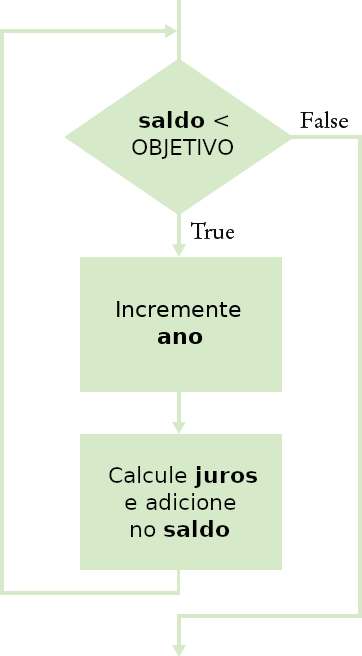
\includegraphics[height=0.65\paperheight,center]{pucrs-ep-fprog-unidade_04-lacos-laminas-fluxograma_laco.png}
\end{figure}
	\end{column}
	\begin{column}{0.7\linewidth}
		\begin{itemize}
		\item Cálculo de juros compostos (Unidade 1)
{\tiny
\begin{minted}[bgcolor=cyan!10]{text}
Inicie com um valor de ano igual a zero e um total de $10.000
Repita o seguinte enquanto o total seja menor do que $20.000
     Adicione 1 ao valor do ano
     Multiplique o total por 1,05 (crescimento de 5%)
Informe o último valor atribuído ao ano como resposta
\end{minted}
}
		\item Em Java:
{\scriptsize
\begin{javacode}
while (saldo < ALVO) {
   ano++;
   double juros = saldo * TAXA_DE_JUROS/100.0;
   saldo = saldo + juros;
}
\end{javacode}
}
		\end{itemize}
	\end{column}
\end{columns}
\end{frame}

%-------------------------------------------------------
\begin{frame}[fragile]\frametitle{\texttt{DobrandoInvestimento.java}}
\tiny{\inputminted[bgcolor=cyan!10]{java}{src/DobrandoInvestimento.java}}
{\tiny
Resultado:
\begin{minted}[bgcolor=cyan!10]{text}
O valor investido dobra após 15 anos.
\end{minted}
}
\end{frame}

%-------------------------------------------------------
\begin{frame}[fragile]\frametitle{Exemplos de Laços com \texttt{while} (1)}
{\scriptsize
\begin{center}
  \begin{tabular}{|p{6cm}|p{2cm}|p{5cm}|}
\hline
    \textbf{Laço} & \textbf{Saída} & \textbf{Explicação} \\
\hline
{\tiny
\begin{minted}{java}
i = 0; soma = 0;
while (soma < 10) {
   i++; soma = soma + i;
   System.out.println(i+" "+soma);
}
\end{minted}
}
&
{\tiny
\begin{verbatim}
1 1
2 3
3 6
4 10
\end{verbatim}
}
& Quando \texttt{soma} for igual a $10$, a condição do laço será falsa, e o laço se encerra.\\
\hline
{\tiny
\begin{minted}{java}
i = 0; soma = 0;
while (soma < 10) {
   i++; soma = soma - i;
   System.out.println(i+" "+soma);
}
\end{minted}
}
&
{\tiny
\begin{verbatim}
1 -1
2 -3
3 -6
4 -10
...
\end{verbatim}
}
& Como \texttt{soma} nunca atinge $10$, isto consiste em um ``laço infinito''.\\
\hline
{\tiny
\begin{minted}{java}
i = 0; soma = 0;
while (soma < 0) {
   i++; soma = soma - i;
   System.out.println(i+" "+soma);
}
\end{minted}
}
&
(Nenhuma saída)
& A condição \texttt{soma < 0} é falsa quando é testada pela primeira vez, e o laço nunca é executado.\\
\hline
  \end{tabular}
\end{center}
}
\end{frame}

%-------------------------------------------------------
\begin{frame}[fragile]\frametitle{Exemplos de Laços com \texttt{while} (2)}
{\scriptsize
\begin{center}
  \begin{tabular}{|p{6cm}|p{2cm}|p{5cm}|}
\hline
    \textbf{Laço} & \textbf{Saída} & \textbf{Explicação} \\
\hline
\begin{minted}{java}
i = 0; soma = 0;
while (soma >= 10) {
   i++; soma = soma + i;
   System.out.println(i+" "+soma);
}
\end{minted}
&
(Nenhuma saída)
& O programador provavelmente pensou: ``Pare quando a soma for pelo menos $10$''. Entretanto a condição do laço controla quando o laço é executado, e não quando ele se encerra.\\
\hline
\begin{minted}{java}
i = 0; soma = 0;
while (soma < 10) ; {
   i++; soma = soma + i;
   System.out.println(i+" "+soma);
}
\end{minted}
&
(Nenhuma saída e o programa nunca termina)
& Observe que o ponto-e-vírgula após o teste do laço faz com que o corpo do laço corresponda a um comando vazio. O programa executará para sempre pois \texttt{soma < 0} e este valor não será atualizado no corpo do laço (comando vazio).\\
\hline
  \end{tabular}
\end{center}
}
\end{frame}

%-------------------------------------------------------
\begin{frame}[fragile]\frametitle{Erros Comuns: NÃO pense ``Já chegamos lá?''}
\begin{itemize}
	\item O corpo do laço somente será executado se a condição de teste for verdadeira
	\item Então a lógica correta é ``Continuo executando o laço?''
	\item Se \texttt{saldo} deve crescer até que alcance \texttt{OBJETIVO}, qual versão executará o corpo do laço corretamente?
\begin{columns}[T]
	\begin{column}{0.5\linewidth}
\begin{javacode}
while (saldo < OBJETIVO) {
   ano++;
   juros  = saldo * TAXA;
   saldo = saldo + juros;
}
\end{javacode}
	\end{column}
	\begin{column}{0.5\linewidth}
\begin{javacode}
while (saldo >= OBJETIVO) {
   ano++;
   juros = saldo * TAXA;
   saldo = saldo + juros;
}
\end{javacode}
	\end{column}
\end{columns}
\end{itemize}
\end{frame}

%-------------------------------------------------------
\begin{frame}[fragile]\frametitle{Erros Comuns: laços infinitos}
\begin{itemize}
	\item O corpo do laço será executado até que a condição de teste se torne falsa
	\item O que acontece se você se esquecer de atualizar a variável de teste?
	\begin{itemize}
		\item \texttt{saldo} é a variável de teste (\texttt{OBJETIVO} é constante)
		\item Seu programa ficará no laço para sempre! (ou até que você pare o programa)
	\end{itemize}
\begin{javacode}
while (saldo < OBJETIVO) {
   ano	++;
   juros = saldo * TAXA;
   // saldo = saldo + juros;
}
\end{javacode}
\end{itemize}
\end{frame}

%-------------------------------------------------------
\begin{frame}[fragile]\frametitle{Erros Comuns: erros de limite}
\begin{itemize}
	\item Uma variável do tipo contadora é frequentemente usada na condição de teste
	\item A variável contadora pode iniciar em 0 ou 1 (programadores frequentemente iniciam contadores com 0)
	\item Se você quer contar 5 dedos, qual código deve ser usado?
\begin{columns}[T]
	\begin{column}{0.5\linewidth}
\begin{javacode}
// Inicia em 0, usa-se <
int dedo = 0;
final int DEDOS = 5;
while (dedo < DEDOS) {
   System.out.println(dedo);
   dedo++;
}
// 0,1,2,3,4
\end{javacode}
	\end{column}
	\begin{column}{0.5\linewidth}
\begin{javacode}
// Inicia em 1, usa-se <=
int dedo = 1;
final int DEDOS = 5;
while (dedo <= DEDOS) {
   System.out.println(dedo);
   dedo++;
}
// 1,2,3,4,5
\end{javacode}
	\end{column}
\end{columns}
\end{itemize}
\end{frame}

%-------------------------------------------------------
\begin{frame}\frametitle{Resumo do Laço \texttt{while}}
\begin{itemize}
	\item Laços com \texttt{while} são usados com grande frequência
	\item Inicialize as variáveis antes do teste
	\item A condição é testada ANTES do corpo do laço
	\begin{itemize}
		\item Isto é chamado pré-teste
		\item A condiçao frequentemene usa uma variável contadora
	\end{itemize}
	\item Algo dentro do corpo do laço deve alterar uma das variáveis usadas no teste
	\item Cuidado com laços infinitos!
\end{itemize}
\end{frame}

%=======================================================
\section{Exercícios}

%-------------------------------------------------------
\begin{frame}\frametitle{Exercícios (1)}	
\begin{enumerate}
	\item Faça laços em Java usando \texttt{while} para mostrar:
	\begin{enumerate}[a]	
		\item Os números inteiros de 1 a 10, inclusive
		\item Os números inteiros de 100 a 200, inclusive.
		\item Os números inteiros de 10 a 1, inclusive, em ordem regressiva.
		\item Os números inteiros de -10 a -50, inclusive.
		\item Os números pares entre \texttt{a} e \texttt{b} (com \texttt{a} $\ge$ \texttt{b}).
		\item As 10 primeiras potências de 2.
	\end{enumerate}
\end{enumerate}
\end{frame}

%-------------------------------------------------------
\begin{frame}[fragile]\frametitle{Exercícios (2)}
\begin{enumerate}
	\setcounter{enumi}{1}
	\item O código a seguir calcula a soma dos dígitos de um número (por exemplo, para 1729 o valor seria 1+7+2+9). Acompanhe a 	execução desse código, instrução por instrução, e mostre como os valores das variáveis \texttt{n}, \texttt{sum} e \texttt{digit} se alteram ao longo da execução.
\begin{javacode}
int n = 1729;
int sum = 0;
while (n > 0) {
   int digit = n % 10;
   sum = sum + digit;
   n = n / 10;
}
System.out.println(sum);
\end{javacode}
\end{enumerate}
\end{frame}
	
%-------------------------------------------------------
\begin{frame}\frametitle{Exercícios (3)}
\begin{enumerate}
	\setcounter{enumi}{2}
	\item Escreva laços \texttt{while} em Java, declarando todas as variáveis utilizadas, para:
	\begin{enumerate}[a]
		\item Ler 20 pares de valores (\texttt{a} e \texttt{b}) escrevendo qual é o maior valor.
		\item Calcular a soma dos valores de 1 até 20.
		\item Mostrar os elementos de uma progressão aritmética de \texttt{n} elementos que inicia em \texttt{a} e tem razão \texttt{r}.
		\item Calcular a soma dos elementos do item anterior.
		\item Mostrar os elementos de uma progressão geométrica de \texttt{n} elementos que inicia em \texttt{a} e tem razão \texttt{r}.
		\item Calcular a soma dos elementos do item anterior.
		\item Calcular o fatorial de um número inteiro lido do terminal.
		\item Ler um número inteiro e escrever se ele é primo ou não.
	\end{enumerate}
\end{enumerate}
\end{frame}

%-------------------------------------------------------
\begin{frame}[fragile]\frametitle{Exercícios (4)}
\begin{enumerate}
	\setcounter{enumi}{3}
	\item Faça o teste de mesa para o trecho de programa em Java a seguir, mostrando todas as alterações de valores nas variáveis declaradas e todas as saídas de terminal, e considerando que os valores lidos do teclado serão respectivamente 2, 4, 3, 2, 0, 2.\\
{\scriptsize
\begin{javacode}
Scanner in = new Scanner(System.in);
int x, a, n, z;

x = in.nextInt();
n = in.nextInt();
while (x > 0) {
   a = 1;
   while (a <= n) {
      z=a*n;
      System.out.println(z);
      a = a + 1;
   }
   x = in.nextInt();
   n = in.nextInt();
}
\end{javacode}
}
\end{enumerate}	
\end{frame}

%=======================================================
\section{O Laço \texttt{for}}

%-------------------------------------------------------
\begin{frame}[fragile]\frametitle{O Laço \texttt{for}}
\begin{itemize}
    \item Em Java, tudo que é feito com \texttt{while} pode ser feito também com \texttt{for}
    \item Mas use laços \texttt{for} quando 
	\begin{itemize}
		\item Houver uma variável de indução com início, atualização e fim claramente identificáveis
		\item For interessante deixar o código mais conciso (controle do laço em uma única linha)
	\end{itemize}
	\item Por exemplo, para fazer o somatório dos números de 1 até 10 poderíamos fazer:
	
\begin{columns}[T]
	\begin{column}{0.5\linewidth}
{\scriptsize
\begin{javacode}
int soma = 0;
// versao com while
int i = 1;  // inicializacao
while (i <= 10)  { // teste
   soma = soma + i;
   i++; // atualizacao
}
\end{javacode}
}
	\end{column}
	\begin{column}{0.5\linewidth}
{\scriptsize
\begin{javacode}
int soma = 0;
// versao com for
for (int i = 1; i <= 10; i++) {
   soma = soma + i;
}
\end{javacode}
}
\end{column}
\end{columns}
\end{itemize}
\end{frame}

%-------------------------------------------------------
\begin{frame}[fragile]\frametitle{Sintaxe do Comando \texttt{for}}
\begin{javacode}
for ( inicializacao; condicao; atualizacao)
    corpo;
\end{javacode}
\begin{itemize}
    \item O comando \texttt{for} tem 4 partes:
    \begin{enumerate}
        \item Inicialização: é executada uma vez antes do laço iniciar
        \item Condição de permanênica: é verificada antes de cada iteração (deve ser verdadeira)
        \item Corpo do laço (bloco de comandos ou comando único): executado enquanto a condição for verdadeira
        \item Atualização: executada sempre depois do bloco de comandos e antes de se fazer um novo teste da condição
    \end{enumerate}
    \item Depois da inicialização, o laço \texttt{for} repetirá um ciclo formado por
    \begin{itemize}
        \item Teste da condição --- Execução do corpo do laço --- Atualização
    \end{itemize}
\end{itemize}
\end{frame}

%-------------------------------------------------------
\begin{frame}\frametitle{Execução de um laço \texttt{for}}
\begin{figure}[h]
	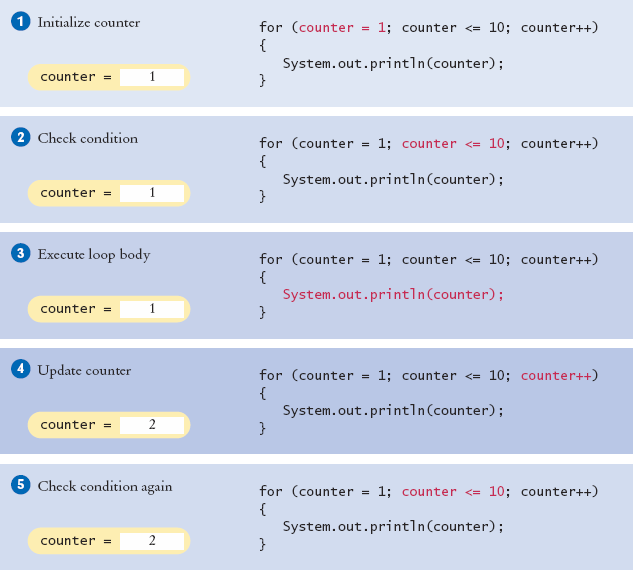
\includegraphics[height=0.70\paperheight,center]{pucrs-ep-fprog-unidade_04-lacos-laminas-execucao_do_laco_for.png}
\end{figure}
\end{frame}

%-------------------------------------------------------
\begin{frame}[fragile]\frametitle{Exemplos de Laços \texttt{for} (1)}
\begin{itemize}
\item Contar de 1 (inclusive) até 5 (inclusive) [5 iterações: 1 2 3 4 5]
{\scriptsize
\begin{javacode}
for (int i = 1; i<=5; i++) System.out.println(i);
for (int i = 1; i<6; i++) System.out.println(i);
\end{javacode}
}
\item Contar de 1 (inclusive) até 5 (exclusive) [4 iterações: 1 2 3 4]
{\scriptsize
\begin{javacode}
for (int i = 1; i<=4; i++) System.out.println(i);
for (int i = 1; i<5; i++) System.out.println(i);
\end{javacode}
}
\item Contar de 0 (inclusive) até 5 (inclusive) [6 iterações: 0 1 2 3 4 5]
{\scriptsize
\begin{javacode}
for (int i = 0; i<=5; i++) System.out.println(i);
for (int i = 0; i<6; i++) System.out.println(i);
\end{javacode}
}
\item Contar de 0 (inclusive) até 5 (exclusive) [5 iterações: 0 1 2 3 4]
{\scriptsize
\begin{javacode}
for (int i = 0; i<=4; i++) System.out.println(i);
for (int i = 0; i<5; i++) System.out.println(i);
\end{javacode}
}
\end{itemize}
\end{frame}

%-------------------------------------------------------
\begin{frame}[fragile]\frametitle{Exemplos de Laços \texttt{for} (2)}
\begin{itemize}
\item Contagem regressiva [6 iterações: 5 4 3 2 1 0]
{\scriptsize
\begin{javacode}
for (int i = 5; i>=0; i--) System.out.println(i);
\end{javacode}
}
\item Incremento igual a 2 [5 iterações: 0 2 4 6 8]
{\scriptsize
\begin{javacode}
for (int i = 0; i<9; i=i+2) System.out.println(i);
\end{javacode}
}
\item Razão geométrica igual a 2 [5 iterações: 1 2 4 8 16]
{\scriptsize
\begin{javacode}
for (int i = 1; i<=20; i=i*2) System.out.println(i);
\end{javacode}
}
\item Percorrer todas as letras de uma cadeia de caracteres [4 iterações: J A V A]
{\scriptsize
\begin{javacode}
String s = "JAVA";
for (int i = 0; i<s.length(); i++) System.out.println(s.charAt(i));
\end{javacode}
}
\end{itemize}
\end{frame}

%-------------------------------------------------------
\begin{frame}[fragile]\frametitle{Planejando um Laço \texttt{for}}
\begin{columns}[T]
	\begin{column}{0.3\linewidth}
\begin{figure}[h]
	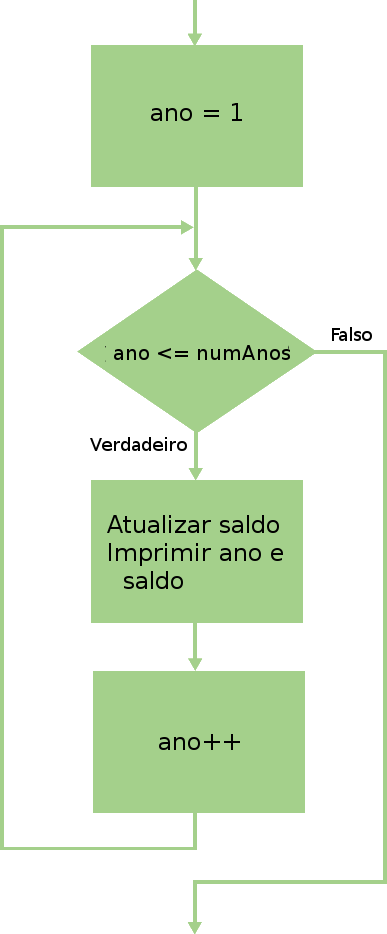
\includegraphics[height=0.70\paperheight,center]{pucrs-ep-fprog-unidade_04-lacos-laminas-fluxograma_laco_for.png}
\end{figure}
	\end{column}
	\begin{column}{0.7\linewidth}
	\begin{itemize}
        {\footnotesize
		\item Considerando um valor inicial investido de 10000, e uma taxa de juros anual de 5\%, escreva um programa que: leia o número total de anos de investimento (\texttt{numAnos}) e, para cada ano transcorrido, imprima o número do ano e o saldo total ao final desse ano.
		\item Por exemplo, para \texttt{numAnos} igual a 5, o programa deve imprimir:
		}
		\begin{itemize}
            {\scriptsize
			\item ano 1: 10500.00
			\item ano 2: 11025.00
			\item ano 3: 11576.25
			\item ano 4: 12155.06
			\item ano 5: 12762.82\\
			}
		\end{itemize}
	\end{itemize}
{\scriptsize
\begin{javacode}
for (int ano = 1; ano <= numAnos; ano++) {
   // Atualiza saldo
   // Imprime ano e saldo
}
\end{javacode}
}
	\end{column}
\end{columns}
\end{frame}

%-------------------------------------------------------
\begin{frame}[fragile]\frametitle{\texttt{Investimento.java}}
\tiny{\inputminted[bgcolor=cyan!10]{java}{src/Investimento.java}}
\end{frame}

%-------------------------------------------------------
\begin{frame}[fragile]\frametitle{Cuidados a serem tomados}
\begin{itemize}
    \item Limite final do laço: inclusive ou exclusive?
    \item Variável de indução: crescente ou decrescente?
    \begin{itemize}
        \item Com valores crescentes usa-se $\le$ ou $<$
        \item Com valores decrescentes usa-se $\ge$ ou $>$
    \end{itemize}
    \item Condições erradas podem gerar \textbf{laços infinitos}:
{\scriptsize
\begin{javacode}
// 0 2 4 6 8 10 ...
for (int i=0; i!=9; i=i+2) System.out.println(i);

// 0 -1 -2 -3 -4 -5 ...
for (int i=0; i<10; --i) System.out.println(i);
\end{javacode}
}
	\item Evite atualizar o contador no corpo do laço \texttt{for}:
{\scriptsize
\begin{javacode}
for (int i=1; i<=100; i++) {
   if (i % 10 == 0)       // Pular valores divisiveis por 10
      i++;                // Estilo ruim para for...
   System.out.println(i);
}
\end{javacode}
}
\end{itemize}
\end{frame}

%-------------------------------------------------------
\begin{frame}[fragile]\frametitle{Escopo de Variáveis do Laço \texttt{for}}
\begin{itemize}
	\item Escopo é o ``tempo de vida'' de uma variável.
	\item Quando a variável \texttt{x} é declarada no comando \texttt{for}, ela existe apenas dentro do bloco do laço
\begin{javacode}
for ( int x = 1; x < 10; x = x + 1) {
   // comandos a serem executados dentro do laco
   // 'x' pode ser usado em qualquer lugar dentro deste bloco
}
if (x > 100)   // Erro! 'x' esta fora de escopo!
\end{javacode}
	\item Solução: declarar 'x' fora do laço
\begin{javacode}
int x;
for ( x = 1; x < 10; x = x + 1) {}
\end{javacode}
\end{itemize}
\end{frame}

%-------------------------------------------------------
\begin{frame}\frametitle{Resumo do Laço \texttt{for}}
\begin{itemize}
	\item Laços com \texttt{for} são muito usados
	\item Eles têm uma notação bastante concisa
	\begin{itemize}
		\item Inicialização ; Condição ; Atualização ; Corpo do laço
		\item A inicialização acontece uma única vez no início do laço
		\item A condição é testada todas as vezes ANTES (pré-teste) de executar o corpo do laço
		\item O incremento é realizado APÓS o corpo do laço
	\end{itemize}
	\item Use laços \texttt{for} seguindo o modelo padrão
	\item Adequado para contagens inteiras, processamento de \emph{strings}, vetores ou matrizes, etc.
\end{itemize}
\end{frame}

%=======================================================
\section{Exercícios sobre Laço \texttt{for}}

%-------------------------------------------------------
\begin{frame}\frametitle{Exercícios 1 e 2}
\begin{enumerate}
    \item Escreva laços \texttt{for} em Java, declarando todas as variáveis utilizadas, para:
    \begin{enumerate}[a.]
        \item Mostrar os valores de 1 até 10.
        \item Mostrar os valores de 10 até 1, em ordem regressiva.
        \item Calcular a soma dos valores de 1 até 20.
        \item Calcular o fatorial de um número inteiro lido do terminal.
        \item Ler 20 pares de valores (\texttt{a} e \texttt{b}) escrevendo qual é o maior valor.
        \item Ler um número inteiro e escrever se ele é primo ou não.
    \end{enumerate}
    \item Escreva um programa em Java para ler o número de alunos de uma turma e a seguir ler as notas destes alunos na prova da disciplina, determinando e imprimindo: a média da turma, a nota mais baixa e a nota mais alta.
\end{enumerate}
\end{frame}

%-------------------------------------------------------
\begin{frame}[fragile]\frametitle{Exercício 3}
\begin{enumerate}
    \setcounter{enumi}{2}
    \item Faça o teste de mesa para o trecho de programa em Java a seguir, mostrando todas as alterações de valores nas variáveis declaradas e todas as saídas de terminal, e considerando que os valores lidos do teclado serão respectivamente 4, 2, 2, 3, 2, 0.
{\scriptsize
\begin{javacode}
Scanner in = new Scanner(System.in);
int x, a, n, z;

n = in.nextInt();
for ( x = in.nextInt() ; x > 0 ; x = in.nextInt() ) {
   for ( a = 1 ; a <= n ; a = a + 1 ) {
      z=a*n;
      System.out.println(z);
   }
   n = in.nextInt();
}
\end{javacode}
}
\end{enumerate}
\end{frame}

%=======================================================
\section{O Laço \texttt{do}}

%-------------------------------------------------------
\begin{frame}[fragile]\frametitle{O Laço \texttt{do}}
\begin{columns}[T]
	\begin{column}{0.3\linewidth}
\begin{figure}[h]
	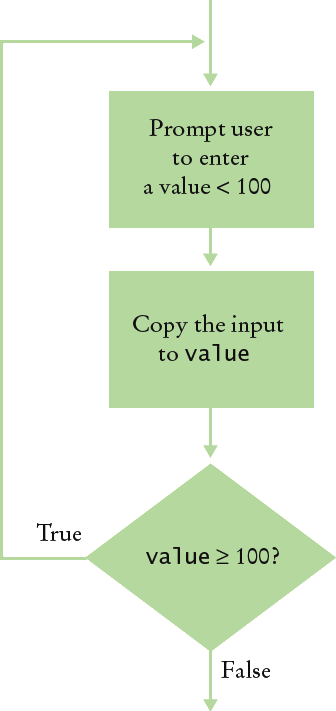
\includegraphics[height=0.65\paperheight,center]{pucrs-ep-fprog-unidade_04-lacos-laminas-fluxograma_laco_do.png}
\end{figure}
	\end{column}
	\begin{column}{0.7\linewidth}
\begin{itemize}
	\item Usa-se o laço \texttt{do} quando se deseja executar o corpo do laço pelo menos uma vez, testando a condição APÓS a primeira repetição do laço
\end{itemize}
\begin{javacode}
int i = 1;  // inicializacao
final int DEDOS = 5;
do {
   // comandos...
   i++; // atualizacao
}  while (i <= DEDOS);  // teste
\end{javacode}
	\end{column}
\end{columns}

\end{frame}

%-------------------------------------------------------
\begin{frame}[fragile]\frametitle{Exemplo de Laço \texttt{do}}
\begin{itemize}
	\item Validação da entrada de usuários
	\begin{itemize}
		\item Verificar se um valor lido está dentro do limite
		\item O usuário tem que fornecer alguma entrada antes para ser validada 
	\end{itemize}
\end{itemize}
\begin{javacode}
int valor;
do {
   System.out.println("Forneca um valor inteiro < 100: "); 
   valor = in.nextInt();
}  while (valor >= 100);  // Teste
\end{javacode}
\end{frame}

%-------------------------------------------------------
\begin{frame}\frametitle{Dica de Programação}
\begin{itemize}
	\item Fluxogramas para laços: evite código "spaghetti" (nunca faça uma seta apontar para dentro do corpo de um laço)
\end{itemize}
\begin{columns}[T]
	\begin{column}{0.5\linewidth}
\begin{center}
\texttt{while} e \texttt{for} testam antes
\begin{figure}[h]
	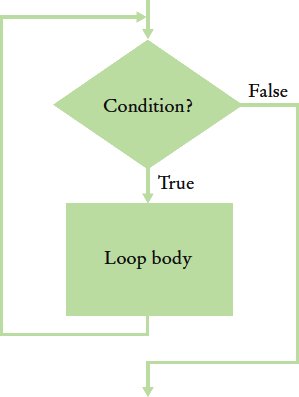
\includegraphics[height=0.4\paperheight,center]{pucrs-ep-fprog-unidade_04-lacos-laminas-fluxograma_teste_antes.png}
\end{figure}
\end{center}
	\end{column}
	\begin{column}{0.5\linewidth}
\begin{center}
\texttt{do} testa depois
\begin{figure}[h]
	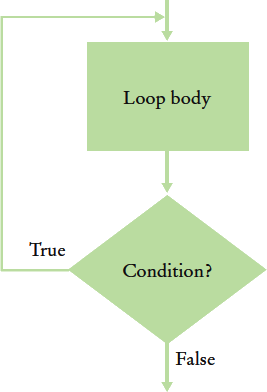
\includegraphics[height=0.4\paperheight,center]{pucrs-ep-fprog-unidade_04-lacos-laminas-fluxograma_teste_depois.png}
\end{figure}
\end{center}
	\end{column}
\end{columns}

\end{frame}

%-------------------------------------------------------
\begin{frame}\frametitle{Humor}
\begin{figure}[h]
	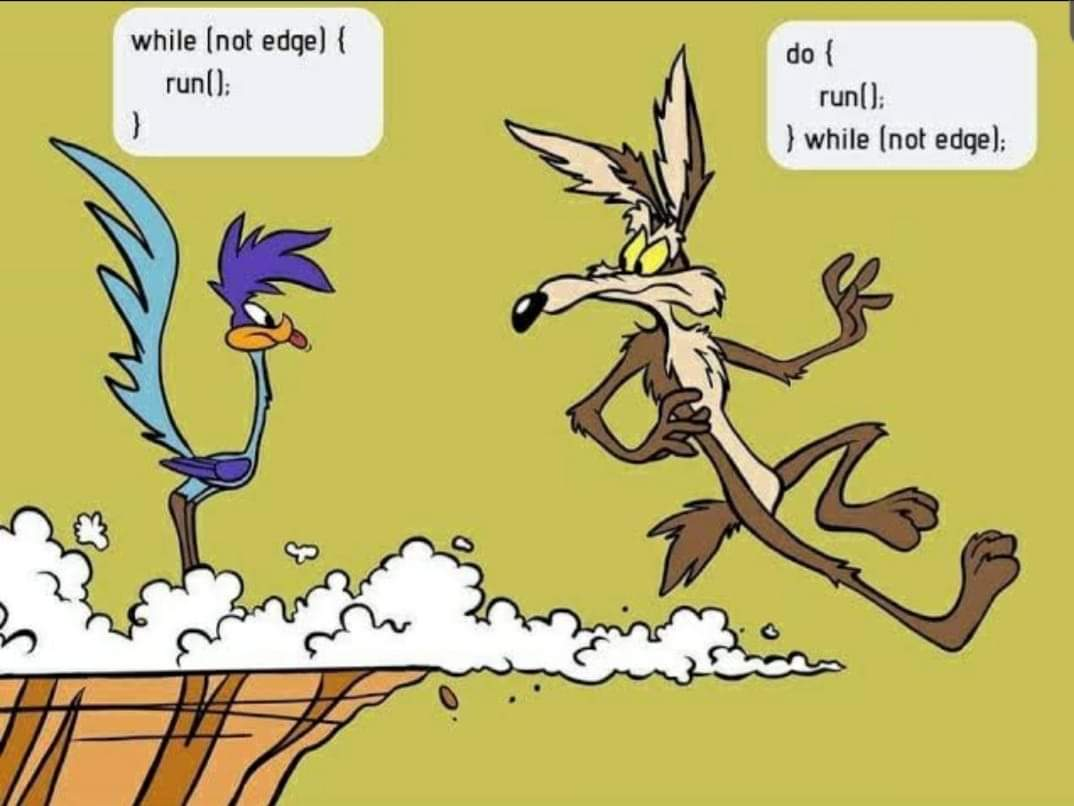
\includegraphics[height=0.7\paperheight,center]{pucrs-ep-fprog-unidade_04-lacos-laminas-while_vs_do_while.jpg}
\end{figure}
\end{frame}

%=======================================================
\section{Sentinelas de Processamento}

%-------------------------------------------------------
\begin{frame}[fragile]\frametitle{Sentinelas de Processamento}
\begin{itemize}
	\item Valores de sentinela indicam o final de um conjunto de dados, mas não fazem parte dos dados
	\item Podem ser usados em muitos casos
	\begin{itemize}
		\item Quando não se sabe quantos itens há em uma lista, usa-se um caracter ou valor especial para sinalizar que não há mais itens
		\item Para entradas de números positivos, é comum usar o valor -1:
\begin{javacode}
int numFuncionarios = 0;
double salario = in.nextDouble();
double soma = 0.0;
while (salario != -1) {
   soma = soma + salario;
   numFuncionarios++;
   salario = in.nextDouble();
}	
\end{javacode}
	\end{itemize}
\end{itemize}
\end{frame}

%-------------------------------------------------------
\begin{frame}\frametitle{Calculando a Média de um Conjunto Indeterminado de Valores}
\begin{itemize}
	\item Declare e inicialize uma variável \texttt{soma} com 0
	\item Declare e inicialize uma variável \texttt{contagem} com 0
	\item Declare e inicialize uma variável \texttt{entrada} com 0
	\item Mostre uma mensagem solicitando que o usuário forneça os dados
	\item Fique no laço até que o valor de sentinela seja fornecido
	\begin{itemize}
		\item Leia um valor e salve em \texttt{entrada}
		\item Se \texttt{entrada} não for igual a -1
		\begin{itemize}
			\item Adicione \texttt{entrada} em \texttt{sum}
			\item Adicione 1 na variável \texttt{contagem}
		\end{itemize}
	\end{itemize}
	\item Tenha certeza de que pelo menos um valor for fornecido antes de fazer a divisão
	\begin{itemize}
		\item Divida \texttt{sum} por \texttt{contagem} e mostre o resultado
	\end{itemize}
	\item Fim	
\end{itemize}
\end{frame}

%-------------------------------------------------------
\begin{frame}[fragile]\frametitle{\texttt{Sentinela.java}}
\tiny{\inputminted[bgcolor=cyan!10]{java}{src/Sentinela.java}}
\end{frame}

%-------------------------------------------------------
\begin{frame}[fragile]\frametitle{Variáveis Booleanas e Sentinelas}
\begin{itemize}
	\item Uma variável booleana (frequentemente chamada de \emph{flag} pode ser usada para controlar um laço)
\begin{javacode}
System.out.print("Forneça um conjunto de valores (use -1 para terminar): ");
boolean concluido = false;
while (!concluido) {
   double valor = in.nextDouble();
   if (valor == -1) {
      concluido = true;
   }
   else {
      // Processa o valor
   }
}
\end{javacode}
\end{itemize}
\end{frame}

%-------------------------------------------------------
\begin{frame}[fragile]\frametitle{Para permitir qualquer valor numérico...}
\begin{itemize}
	\item Se os valores válidos puderem ser negativos ou positivos, não se pode usar -1 (ou qualquer outro número) como sentinela
	\item A solução então é usar qualquer outra sentinela não numérica
	\item Como \texttt{in.nextDouble} falha para valores não numéricos, deve-se usar \texttt{in.hasNextDouble} antes
	\begin{itemize}
		\item Retorna um booleano: \texttt{true}, se a entrada estiver correta (for um número), ou \texttt{false}, se a entrada não for um número
		\item Em caso de \texttt{true}, pode-se usar \texttt{in.nextDouble}
	\end{itemize}
\begin{javacode}
System.out.print("Forneça valores reais (digite Q para encerrar): ");
while (in.hasNextDouble()) {
   double valor = in.nextDouble();
   // Processa o valor...
}
\end{javacode}
\end{itemize}
\end{frame}

%=======================================================
\section{Algoritmos Comuns com Laços}

%-------------------------------------------------------
\begin{frame}\frametitle{Algoritmos Comuns com Laços}
\begin{itemize}
	\item Somatório
	\item Produtório
	\item Valor médio
	\item Contagem de ocorrências
	\item Encontrar a primeira ocorrência
	\item Perguntar até que uma ocorrência seja encontrada
	\item Máximo e mínimo
	\item Comparar valores adjacentes
\end{itemize}
\end{frame}

%-------------------------------------------------------
\begin{frame}[fragile]\frametitle{Somatório}
\begin{itemize}
	\item Inicialize \texttt{total} com 0
	\item Pode-se usar o laço com sentinela
	\item Acrescente o valor em \texttt{total}
\end{itemize}
\begin{javacode}
double total = 0;
while (in.hasNextDouble()) {
   double entrada = in.nextDouble();
   total = total + entrada;
}
\end{javacode}
\end{frame}

%-------------------------------------------------------
\begin{frame}[fragile]\frametitle{Produtório}
\begin{itemize}
	\item Inicialize \texttt{produto} com 1
	\item Mutiplique o valor por \texttt{produto}
\end{itemize}
\begin{javacode}
double produto = 1;
while (in.hasNextDouble()) {
   double entrada = in.nextDouble();
   produto = produto * entrada;
}
\end{javacode}
\end{frame}

%-------------------------------------------------------
\begin{frame}[fragile]\frametitle{Valor Médio}
\begin{itemize}
	\item Faça o somatório dos valores
	\item Inicialize \texttt{contagem} com 0, incrementando-a a cada valor lido
	\item Verifique o valor de \texttt{contagem} antes da divisão!
\end{itemize}
{\footnotesize
\begin{javacode}
double total = 0;
int contagem = 0;
while (in.hasNextDouble()) {
   double entrada = in.nextDouble();
   total = total + entrada;
   contagem++;
}
if (contagem > 0) {
   double media = total / contagem;
   System.out.println("Media = " + media);
}
\end{javacode}
}
\end{frame}

%-------------------------------------------------------
\begin{frame}[fragile]\frametitle{Contagem de Ocorrências}
\begin{itemize}
	\item Inicialize \texttt{contagem} com 0
	\item Use um laço \texttt{for}
	\item Incremente o contador a cada ocorrência
\end{itemize}
\begin{javacode}
int letrasMaiusculas = 0;
for (int i = 0; i < str.length(); i++) {
   char ch = str.charAt(i);
   if (Character.isUpperCase(ch)) {
      letrasMaiusculas++;
   }
}
\end{javacode}
\end{frame}

%-------------------------------------------------------
\begin{frame}[fragile]\frametitle{Encontrar a Primeira Ocorrência}
\begin{itemize}
	\item Inicialize uma variável sentinela/booleana com \texttt{false}
	\item Inicialize o contador de posições com 0 (primeiro caracter do \emph{string})
	\item Use uma condição composta no laço
	\item Laços com pré-teste tratam a situação para \emph{string} vazio
\end{itemize}
{\footnotesize
\begin{javacode}
boolean found = false;
char ch;
int position = 0;
while (!found && position < str.length()) {
   ch = str.charAt(position);
   if (Character.isLowerCase(ch)) { 
      found = true; 
   }
   else { position++; }
}
\end{javacode}
}
\end{frame}

%-------------------------------------------------------
\begin{frame}[fragile]\frametitle{Perguntar até que uma Ocorrência Seja Encontrada}
\begin{itemize}
	\item Inicialize uma variável sentinela/booleana com \texttt{false}
	\item Teste a variável sentinela no laço \texttt{while}
	\begin{itemize}
		\item Leia a entrada, e compare com o limite
		\item Se a entrada está dentro do limite, altere a variável sentinela para \texttt{true}
		\item O laço parará de executar
	\end{itemize}
\end{itemize}
{\footnotesize
\begin{javacode}
boolean valido = false;
double entrada;
while (!valido) {
   System.out.print("Forneça um valor positivo < 100: ");
   entrada = in.nextDouble();
   if (0 < entrada && entrada < 100) { valido = true; }
   else { System.out.println("Entrada inválida!"); }
}
\end{javacode}
}
\end{frame}

%-------------------------------------------------------
\begin{frame}[fragile]\frametitle{Máximo e Mínimo}
\begin{itemize}
	\item Leia o primeiro valor: este é o maior (ou menor) valor que você obteve até agora!
	\item Fique no laço enquanto você tiver um valor válido
	\begin{itemize}
		\item Leia outro valor
		\item Compare o novo valor com o maior (ou menor)
		\item Atualize o maior (ou menor) valor se for necessário
	\end{itemize}
\end{itemize}
\begin{columns}[T]
	\begin{column}{0.5\linewidth}
{\footnotesize
\begin{javacode}
double maior = in.nextDouble();
while (in.hasNextDouble()) {
   double valor = in.nextDouble();
   if (valor > maior) {
      maior = valor;
   }
}
\end{javacode}
}
	\end{column}
	\begin{column}{0.5\linewidth}
{\footnotesize
\begin{javacode}
double menor = in.nextDouble();
while (in.hasNextDouble()) {
   double valor = in.nextDouble();
   if (valor < menor) {
      menor = valor;
   }
}
\end{javacode}
}
	\end{column}
\end{columns}
\end{frame}

%-------------------------------------------------------
\begin{frame}[fragile]\frametitle{Comparar Valores Adjacentes}
\begin{itemize}
	\item Obtenha o primeiro valor da entrada
	\item Use o \texttt{while} para determinar se há mais valores para serem verificados
	\begin{itemize}
		\item Copie a entrada para uma variável para armazenar o valor anterior		
		\item Leia a próxima entrada
		\item Compare a entrada lida com o valor anterior, e avise se forem iguais
	\end{itemize}
\end{itemize}
%{\footnotesize
\begin{javacode}
double entrada = in.nextDouble();
while (in.hasNextDouble()) {
   double anterior = entrada;
   entrada = in.nextDouble();
   if (entrada == anterior) { 
      System.out.println("Entrada duplicada!"); 
   }
}
\end{javacode}
%}
\end{frame}

%-------------------------------------------------------
\begin{frame}\frametitle{Passos para Escrever um Laço}
Planejamento:
\begin{itemize}
	\item Decida que tarefa realizar dentro do laço
	\item Especifique a condição do laço
	\item Determine o tipo do laço
	\item Inicialize as variáveis antes da primeira iteração
	\item Processe os resultados depois que o laço tenha encerrado
	\item Teste o laço com exemplos típicos
\end{itemize}
Codificação:
\begin{itemize}
	\item Implemente o laço em Java
\end{itemize}
\end{frame}

%=======================================================
\section{Laços Aninhados}

%-------------------------------------------------------
\begin{frame}\frametitle{Laços Aninhados}
\begin{columns}[T]
	\begin{column}{0.5\linewidth}
\begin{itemize}
	\item Como você imprimiria uma tabela com linhas e colunas?
	\begin{itemize}
		\item Imprima a primeira linha com o cabeçalho
		\begin{itemize}
			\item Use um laço
		\end{itemize}
		\item Imprima o corpo da tabela
		\begin{itemize}
			\item Quantas linhas?
			\item Quantas colunas?
		\end{itemize}
		\item Faça um laço para as linhas
		\begin{itemize}
			\item Faça um laço para as colunas
		\end{itemize}
	\end{itemize}
\end{itemize}
	\end{column}
	\begin{column}{0.5\linewidth}
\begin{figure}[h]
	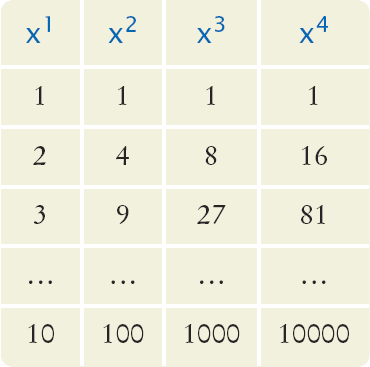
\includegraphics[height=0.5\paperheight,center]{pucrs-ep-fprog-unidade_04-lacos-laminas-tabela.png}
\end{figure}
	\end{column}
\end{columns}
\end{frame}

%-------------------------------------------------------
\begin{frame}\frametitle{Fluxograma de Dois Laços Aninhados}
\begin{figure}[h]
	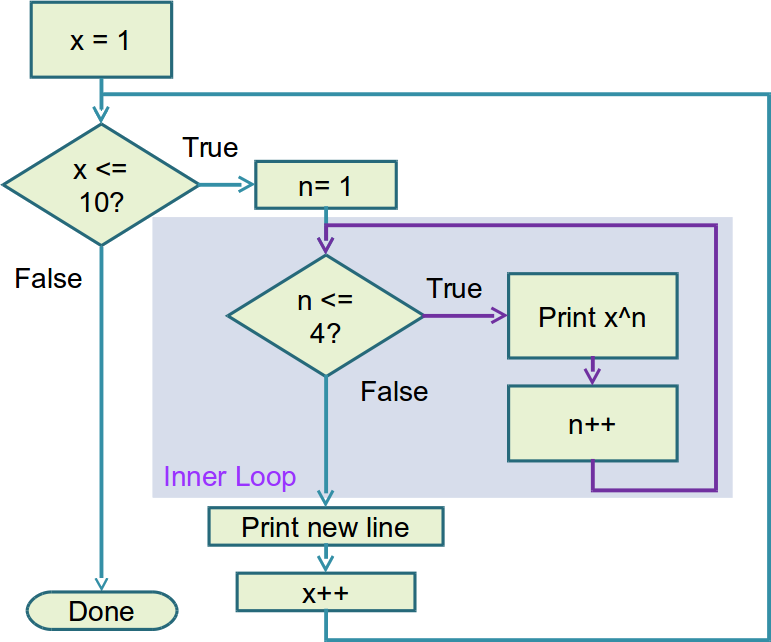
\includegraphics[height=0.65\paperheight,center]{pucrs-ep-fprog-unidade_04-lacos-laminas-fluxograma_lacos_aninhados.png}
\end{figure}
\end{frame}

%-------------------------------------------------------
\begin{frame}[fragile]\frametitle{\texttt{TabelaDePotencias.java}}
\tiny{\inputminted[bgcolor=cyan!10]{java}{src/TabelaDePotencias.java}}
\end{frame}

%-------------------------------------------------------
\begin{frame}\frametitle{Resultado de \texttt{TabelaDePotencias.java}}
\begin{figure}[h]
	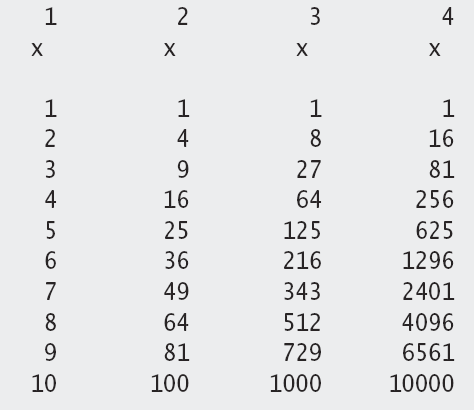
\includegraphics[height=0.65\paperheight,center]{pucrs-ep-fprog-unidade_04-lacos-laminas-resultado_de_powertable.png}
\end{figure}
\end{frame}

%-------------------------------------------------------
\begin{frame}[fragile]\frametitle{Exercício}
Modifique o programa \texttt{TabelaDePotencias.java} para que a tabela seja impressa ``deitada'', ou seja, na primeira linha os valores para $x^1$, na segunda linha os valores para $x^2$, e assim por diante.
\end{frame}

%-------------------------------------------------------
\begin{frame}[fragile]\frametitle{Exemplos de Laços Aninhados (1)}
\begin{center}
  \begin{tabular}{|p{6cm}|p{2cm}|p{5cm}|}
\hline
    \textbf{Laço} & \textbf{Saída} & \textbf{Explicação} \\
\hline
{\tiny
\begin{minted}{java}
for (i = 1; i <= 3 ; i++) {
   for (j = 1; j <= 4; j++) {
      System.out.print("*");
   }
   System.out.println();
}
\end{minted}
}
&
{\tiny
\begin{verbatim}
****
****
****
\end{verbatim}
}
& Imprime 3 linhas de 4 asteriscos cada.\\
\hline
{\tiny
\begin{minted}{java}
for (i = 1; i <= 4 ; i++) {
   for (j = 1; j <= 3; j++) {
      System.out.print("*");
   }
   System.out.println();
}
\end{minted}
}
&
{\tiny
\begin{verbatim}
***
***
***
***
\end{verbatim}
}
& Imprime 4 linhas de 3 asteriscos cada.\\
\hline
  \end{tabular}
\end{center}
\end{frame}

%-------------------------------------------------------
\begin{frame}[fragile]\frametitle{Exemplos de Laços Aninhados (2)}
\begin{center}
  \begin{tabular}{|p{6cm}|p{2cm}|p{5cm}|}
\hline
    \textbf{Laço} & \textbf{Saída} & \textbf{Explicação} \\
\hline
{\tiny
\begin{minted}{java}
for (i = 1; i <= 4 ; i++) {
   for (j = 1; j <= i; j++) {
      System.out.print("*");
   }
   System.out.println();
}
\end{minted}
}
&
{\tiny
\begin{verbatim}
*
**
***
****
\end{verbatim}
}
& Imprime 4 linhas com tamanhos 1, 2, 3 e 4.\\
\hline
{\tiny
\begin{minted}{java}
for (i = 1; i <= 3 ; i++) {
   for (j = 1; j <= 5; j++) {
      if (j % 2 == 0) {
         System.out.print("*");
      }
      else {
         System.out.print("-");
      }
   }
   System.out.println();
}
\end{minted}
}
&
{\tiny
\begin{verbatim}
-*-*-
-*-*-
-*-*-
\end{verbatim}
}
& Imprime asteriscos nas colunas pares e traços nas colunas ímpares.\\
\hline
  \end{tabular}
\end{center}
\end{frame}

%-------------------------------------------------------
\begin{frame}[fragile]\frametitle{Exemplos de Laços Aninhados (3)}
\begin{center}
  \begin{tabular}{|p{6cm}|p{2cm}|p{5cm}|}
\hline
    \textbf{Laço} & \textbf{Saída} & \textbf{Explicação} \\
\hline
{\tiny
\begin{minted}{java}
for (i = 1; i <= 3 ; i++) {
   for (j = 1; j <= 5; j++) {
      if (i % 2 == j % 2) {
         System.out.print("*");
      }
      else {
         System.out.print(" ");
      }
   }
   System.out.println();
}
\end{minted}
}
&
{\tiny
\begin{verbatim}
* * *
 * * 
* * *
\end{verbatim}
}
& Imprime o padrão de um tabuleiro de damas.\\
\hline
  \end{tabular}
\end{center}
\end{frame}

%-------------------------------------------------------
\begin{frame}[fragile]\frametitle{Exercício: faça laços aninhados para imprimir os seguintes padrões}
{\tiny
\begin{columns}[T]
	\begin{column}{0.2\linewidth}
\begin{enumerate}[a)]
	\item	
\begin{verbatim}
*......
.*.....
..*....
...*...
....*..
.....*.
......*

\end{verbatim}
	\item
\begin{verbatim}
*******
.******
..*****
...****
....***
.....**
......*

\end{verbatim}
	\item
\begin{verbatim}
.......
*......
**.....
***....
****...
*****..
******.
\end{verbatim}
\end{enumerate}
	\end{column}
	\begin{column}{0.2\linewidth}
\begin{enumerate}[a)]
  \setcounter{enumi}{3}
	\item
\begin{verbatim}
......*
.....*.
....*..
...*...
..*....
.*.....
*......

\end{verbatim}
	\item
\begin{verbatim}
*******
******.
*****..
****...
***....
**.....
*......

\end{verbatim}
	\item
\begin{verbatim}
......*
.....**
....***
...****
..*****
.******
*******
\end{verbatim}
\end{enumerate}
	\end{column}
	\begin{column}{0.2\linewidth}
\begin{enumerate}[a)]
  \setcounter{enumi}{6}
	\item
\begin{verbatim}
*******
.*****.
..***..
...*...
.......
.......
.......

\end{verbatim}
	\item
\begin{verbatim}
*.....*
.*...*.
..*.*..
...*...
..*.*..
.*...*.
*.....*

\end{verbatim}
	\item
\begin{verbatim}
.......
.......
.......
...*...
..***..
.*****.
*******
\end{verbatim}
\end{enumerate}
	\end{column}
	\begin{column}{0.2\linewidth}
\begin{enumerate}[a)]
  \setcounter{enumi}{9}
	\item
\begin{verbatim}
*******
*.....*
*.....*
*.....*
*.....*
*.....*
*******

\end{verbatim}
	\item
\begin{verbatim}
...*...
...*...
...*...
*******
...*...
...*...
...*...

\end{verbatim}
	\item
\begin{verbatim}
*..*..*
.*.*.*.
..***..
*******
..***..
.*.*.*.
*..*..*
\end{verbatim}
\end{enumerate}
	\end{column}
	\begin{column}{0.2\linewidth}
\begin{enumerate}[a)]
  \setcounter{enumi}{12}
	\item
\begin{verbatim}
*......
**.....
*.*....
*..*...
*...*..
*....*.
*******

\end{verbatim}
	\item
\begin{verbatim}
......*
.....**
....*.*
...*..*
..*...*
.*....*
*******

\end{verbatim}
	\item
\begin{verbatim}
*******
*....*.
*...*..
*..*...
*.*....
**.....
*......
\end{verbatim}
\end{enumerate}
	\end{column}\end{columns}
}
\end{frame}

%=======================================================
\section{Resumo}

%-------------------------------------------------------
\begin{frame}\frametitle{Resumo (1)}
\begin{itemize}
	\item Há 3 tipos de laços:
	\begin{itemize}
		\item Laços \texttt{while}
		\item Laços \texttt{for}
		\item Laços \texttt{do}
	\end{itemize}
	\item Cada laço possui as seguintes seções:
	\begin{itemize}
		\item Inicialização (preparação das variáveis para iniciar o laço)
		\item Condição (teste para verificar se o corpo do laço deve ser executado)
		\item Atualização (alteração de alguma variável testada na condição)
	\end{itemize}
\end{itemize}
\end{frame}

%-------------------------------------------------------
\begin{frame}\frametitle{Resumo (2)}
\begin{itemize}
	\item Um laço executa instruções repetidamente enquanto uma condição for verdadeira
	\item Errar o número de iterações em laço por uma unidade é um erro comum de programação
	\begin{itemize}
		\item Procure deixar os testes simples para evitar este tipo de erro.
	\end{itemize}
	\item O laço \texttt{for} é usado quando um valor varia de um ponto de partida até um ponto final com um incremento ou decremento constante
	\item O laço \texttt{do} é apropriado quando o corpo do laço deve ser executado pelo menos uma vez
\end{itemize}
\end{frame}

%-------------------------------------------------------
\begin{frame}\frametitle{Resumo (3)}
\begin{itemize}
	\item Um valor de sentinela consiste de um valor que determina o final de um conjunto de dados, mas que não faz parte deste conjunto
	\item Você pode usar uma variável booleana para controlar um laço
	\begin{itemize}
		\item Defina a variável com \texttt{true} antes de entrar no laço, e então defina ela com \texttt{false} para sair do laço
	\end{itemize}
	\item Quando o corpo de um laço contiver outro laço, os laços são aninhados
	\begin{itemize}
		\item Um uso típico para laços aninhados é a impressão de uma tabela com linhas e colunas
	\end{itemize}
	\item Em uma simulação, o computador é usado para simular uma atividade
	\begin{itemize}
		\item Pode-se introduzir aleatoriedade chamando o gerador de números aleatórios
	\end{itemize}
\end{itemize}
\end{frame}

%=======================================================
\section{Tópicos Avançados}

%-------------------------------------------------------
\begin{frame}[fragile]\frametitle{Tópicos Avançados}
\begin{itemize}
	\item Números Aleatórios e Simulações
	\item \emph{Storyboards} para resolução de problemas
	\item Gráficos em Java
\end{itemize}
\end{frame}

%-------------------------------------------------------
\begin{frame}\frametitle{Números Aleatórios e Simulações}
\begin{itemize}
	\item Jogos frequentemente usam números aleatórios para tornar as coisas mais interessantes
	\begin{itemize}
		\item Jogar dados
		\item Girar uma roda
		\item ``Comprar'' uma carta
	\end{itemize}
	\item Uma simulação usualmente envolve executar um laço para uma sequência de eventos
	\begin{itemize}
		\item Dias
		\item Eventos
	\end{itemize}
\end{itemize}
\end{frame}

%-------------------------------------------------------
\begin{frame}[fragile]\frametitle{Números Aleatórios e Simulações: \texttt{RandomDemo.java}}
\begin{itemize}
	\item \texttt{Math.random()} pode ser usado para gerar números aleatórios no intervalo [0;1)
\end{itemize}
\begin{columns}[T]
	\begin{column}{0.74\linewidth}
		\scriptsize{\inputminted[bgcolor=cyan!10]{java}{src/RandomDemo.java}}
	\end{column}
	\begin{column}{0.26\linewidth}
{\scriptsize
Resultado:
\begin{minted}[bgcolor=cyan!10]{text}
0,30625248942272576000
0,57255173336825820000
0,38359344863509290000
0,67094454250114250000
0,46419930546834340000
0,45408986890317440000
0,18747367004920823000
0,36019379208793400000
0,02052469620947972000
0,59019359111533320000
\end{minted}
}
	\end{column}
\end{columns}
\end{frame}

%-------------------------------------------------------
\begin{frame}[fragile]\frametitle{Números Aleatórios e Simulações: lançamento de dados}
\begin{itemize}
	\item Pode-se simular o lançamento de dados usando \texttt{Math.random()}
\end{itemize}
\begin{columns}[T]
	\begin{column}{0.8\linewidth}
		\scriptsize{\inputminted[bgcolor=cyan!10]{java}{src/Dados1.java}}
	\end{column}
	\begin{column}{0.2\linewidth}
{\scriptsize
Resultado:
\begin{minted}[bgcolor=cyan!10]{text}
5 1
2 1
1 2
5 1
1 2
6 4
4 4
6 1
6 3
5 2
\end{minted}
}
	\end{column}
\end{columns}
\end{frame}

%-------------------------------------------------------
\begin{frame}[fragile]\frametitle{Números Aleatórios e Simulações: \texttt{Dados2.java}}
\begin{itemize}
	\item Também é possível usar a classe \texttt{Random}, que tem muitos métodos para gerar números aleatórios em diferentes formatos
\scriptsize{\inputminted[bgcolor=cyan!10]{java}{src/Dados2.java}}
\end{itemize}	
\end{frame}

%-------------------------------------------------------
\begin{frame}\frametitle{Números Aleatórios e Simulações: o método de Monte Carlo}
\begin{itemize}
	\item Usado para encontrar soluções aproximadas para problemas que não podem ser resolvidos com precisão
	\item Exemplo: aproximar o valor de PI usando áreas relativas de um círculo dentro de um quadrado
	\begin{itemize}
		\item Usa aritmética simples
		\item Acertos estão dentro do círculo
		\item Lançamentos são o número total de tentativas
		\item Razão é 4 x Acertos / Lançamentos
	\end{itemize}
\begin{figure}[h]
	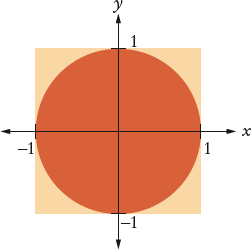
\includegraphics[height=0.2\paperheight,center]{pucrs-ep-fprog-unidade_04-lacos-laminas-monte_carlo.png}
\end{figure}
\end{itemize}
\end{frame}

%-------------------------------------------------------
\begin{frame}[fragile]\frametitle{Números Aleatórios e Simulações: \texttt{MonteCarlo.java}}
\tiny{\inputminted[bgcolor=cyan!10]{java}{src/MonteCarlo.java}}
{\tiny
Resultado:
\begin{minted}[bgcolor=cyan!10]{text}
Estimativa de pi: 3.1452	
\end{minted}
}
\end{frame}

%-------------------------------------------------------
\begin{frame}\frametitle{\emph{Storyboards} para resolução de problemas}
\begin{itemize}
	\item Um storyboard (esboço sequencial) consiste numa sequência de desenhos anotados para cada etapa de uma sequência de ações
	\item Trata-se de uma técnica útil para solução de problemas que permite modelar a interação com o usuário
	\item Pode ajudar a responder:
	\begin{itemize}
		\item Qual informação o usuário deve fornecer e em que ordem?
		\item Qual informação o programa deve mostrar e em que formato?
		\item O que deve acontecer se houver um erro?
		\item Quando o programa deve terminar?
	\end{itemize}
\end{itemize}
\end{frame}

%-------------------------------------------------------
\begin{frame}\frametitle{\emph{Storyboards}: exemplo}
\begin{itemize}
	\item Objetivo: converter uma sequência de medidas
	\begin{itemize}
		\item Exigirá um laço e algumas variáveis
		\item Deverá gerenciar uma conversão de cada vez através de um laço
	\end{itemize}
\begin{figure}[h]
	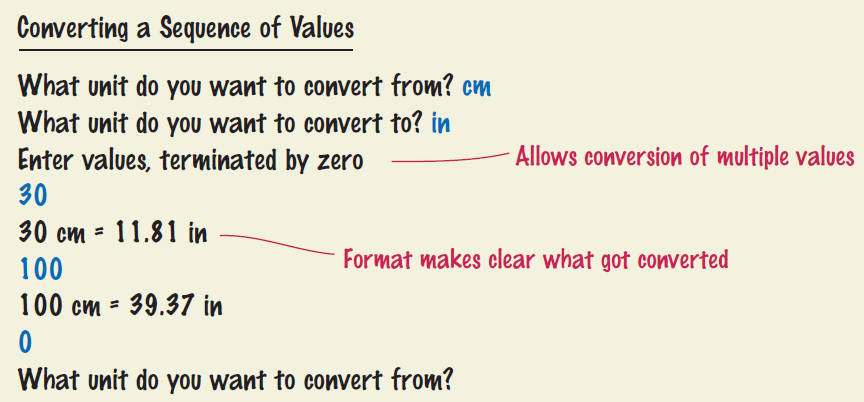
\includegraphics[height=0.5\paperheight,center]{pucrs-ep-fprog-unidade_04-lacos-laminas-storyboards1.jpg}
\end{figure}
\end{itemize}
\end{frame}

%-------------------------------------------------------
\begin{frame}\frametitle{\emph{Storyboards}: o que pode dar errado?}
\begin{itemize}
	\item Unidades de medidas desconhecidas
	\begin{itemize}
		\item Como centímetros e polegadas são digitados?
		\item Que outras conversões estão disponíveis?
	\end{itemize}
	\item Solução: mostra uma lista de tipos de unidades aceitáveis
\begin{figure}[h]
	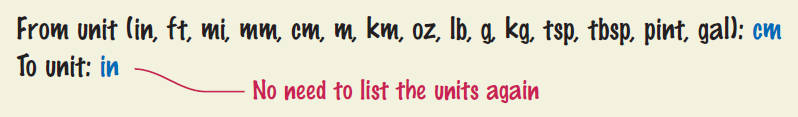
\includegraphics[height=0.15\paperheight,center]{pucrs-ep-fprog-unidade_04-lacos-laminas-storyboards2.jpg}
\end{figure}
\end{itemize}
\end{frame}

%-------------------------------------------------------
\begin{frame}\frametitle{\emph{Storyboards}: o que mais pode dar errado?}
\begin{itemize}
	\item Como o usuário encerra o programa?
\begin{figure}[h]
	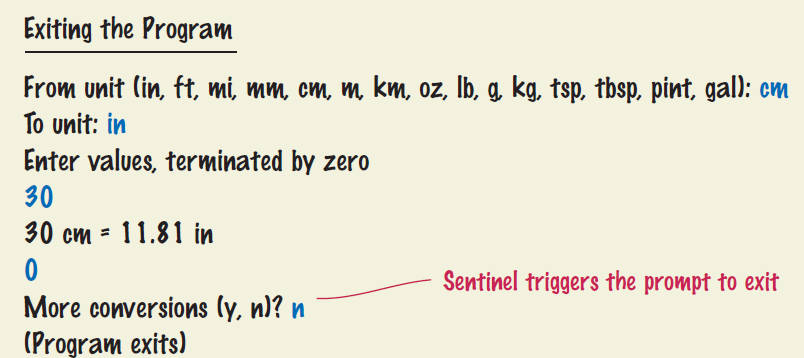
\includegraphics[height=0.5\paperheight,center]{pucrs-ep-fprog-unidade_04-lacos-laminas-storyboards3.jpg}
\end{figure}
	\item Storyboards ajudam a planejar um programa: conhecer os fluxos ajuda a estruturar o código
\end{itemize}
\end{frame}

%-------------------------------------------------------
\begin{frame}\frametitle{Gráficos em Java}
\begin{itemize}
	\item Na sequêncica aparecem algumas dicas sobre como criar programas em Java que utilizam formas geométricas básicas
	\item O objetivo é apenas ter um programa com uma estrutura simples a partir da qual se possa desenhar algumas formas geométricas
	\item NÃO se pretende aprofundar a discussão sobre as classes usadas para criar e controlar janelas em uma \emph{Graphic User Interface} (GUI)
\end{itemize}
\end{frame}

%-------------------------------------------------------
\begin{frame}\frametitle{Gráficos em Java: no método \texttt{main}}
\begin{itemize}
	\item Inicia-se criando um objeto chamado \texttt{frame} da classe \texttt{JFrame}
	\item Um \texttt{JFrame} corresponde a uma moldura dentro da qual se podem colocar ou desenhar outros componentes (no exemplo a seguir, a moldura ou janela será de 400 por 400 \emph{pixels})
	\item Para este \emph{frame}, define-se então o tamanho (chamada ao método \texttt{setSize}) e a operação de fechamento padrão (chamada ao método \texttt{setDefaultCloseOperation})
	\item Em seguida cria-se um componente (\texttt{JComponent}), definindo para este componente um método para desenhar a janela (basicamente este método, que se chama \texttt{paintComponent}, chama o método \texttt{draw}, que será responsável por desenhar a janela)
	\item Adiciona-se o componente ao \emph{frame} (chamada de método \texttt{add})
	\item E, por fim, torna-se o frame \emph{visível} (chamada de método \texttt{setVisible})
\end{itemize}
\end{frame}

%-------------------------------------------------------
\begin{frame}\frametitle{Gráficos em Java: no método \texttt{draw}}
\begin{itemize}
	\item É este método que efetivamente desenha as figuras geométricas na janela (e deve ser declarado como \texttt{static} para poder ser chamado a partir de \texttt{main})
	\item O método \texttt{draw} tem como parâmetro um objeto da classe \texttt{Graphics}
	\item A classe \texttt{Graphics} possui uma série de métodos com os quais se pode desenhar diferentes figuras geométricas (retângulos, elipses, segmentos de reta, etc.)
	\item Pode-se considerar que os objetos da classe \texttt{Graphics} funcionam de forma semelhante a \texttt{System.out}, porém desenhando figuras em um \emph{frame} e não textos em um terminal
	\item No exemplo a seguir, o método \texttt{setColor} define a cor padrão de impressão como sendo azul, e \texttt{fillRect} é usado para desenhar duas fileiras com quadrados preenchidos de forma alternada
	\end{itemize}
\end{frame}

%-------------------------------------------------------
\begin{frame}\frametitle{Gráficos em Java: exemplo}
\begin{itemize}
	\item O exemplo a seguir desenha duas fileiras de retângulos alternados em uma janela
\begin{figure}[h]	
	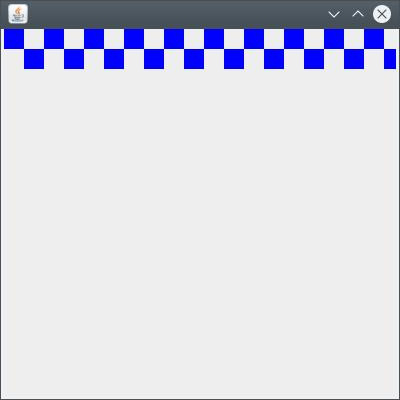
\includegraphics[height=0.6\paperheight,center]{pucrs-ep-fprog-unidade_04-lacos-laminas-exemplo.jpg}
\end{figure}
\end{itemize}
\end{frame}

%-------------------------------------------------------
\begin{frame}[fragile]\frametitle{Gráficos em Java: \texttt{LinhasDeQuadrados.java} {\tiny [Adaptado de Horstmann (2013, p. 180-181)]}}
\tiny{\inputminted[bgcolor=cyan!10]{java}{src/LinhasDeQuadrados.java}}
\end{frame}

%-------------------------------------------------------
\begin{frame}[fragile]\frametitle{Gráficos em Java: alguns métodos de \texttt{Graphics} (1)}
{\scriptsize
\begin{center}
  \begin{tabular}{|p{6cm}|p{3cm}|p{4cm}|}
\hline
    \textbf{Método} & \textbf{Resultado} & \textbf{Explicação} \\
\hline
\texttt{g.drawRect(x, y, width, height)}
&
\begin{figure}[h]
	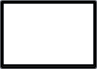
\includegraphics[height=0.1\paperheight,center]{pucrs-ep-fprog-unidade_04-lacos-laminas-retangulo.png}
\end{figure}
& \texttt{(x, y)} é o canto superior esquerdo.\\
\hline
\texttt{g.drawOval(x, y, width, height)}
&
\begin{figure}[h]
	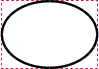
\includegraphics[height=0.1\paperheight,center]{pucrs-ep-fprog-unidade_04-lacos-laminas-elipse.png}
\end{figure}
& \texttt{(x, y)} é o canto superior esquerdo do retângulo que limita a elipse. Para desenhar um cículo usa-se o mesmo valor para \texttt{width} e \texttt{height}.\\
\hline
\texttt{g.fillRect(x, y, width, height)}
&
\begin{figure}[h]
	
\includegraphics[height=0.1\paperheight,center]{pucrs-ep-fprog-unidade_04-lacos-laminas-retangulo_preenchido.png}
\end{figure}
& O retângulo é desenhado preenchido.\\
\hline
  \end{tabular}
\end{center}
}
\end{frame}

%-------------------------------------------------------
\begin{frame}[fragile]\frametitle{Gráficos em Java: alguns métodos de \texttt{Graphics} (2)}
{\scriptsize
\begin{center}
  \begin{tabular}{|p{6cm}|p{3cm}|p{4cm}|}
\hline
    \textbf{Método} & \textbf{Resultado} & \textbf{Explicação} \\
\hline
\texttt{g.fillOval(x, y, width, height)}
&
\begin{figure}[h]
	
\includegraphics[height=0.1\paperheight,center]{pucrs-ep-fprog-unidade_04-lacos-laminas-elipse_preenchida.png}
\end{figure}
& A elipse é desenhada preenchida.\\
\hline
\texttt{g.drawLine(x1, y1, x2, y2)}
&
\begin{figure}[h]
	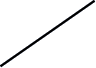
\includegraphics[height=0.1\paperheight,center]{pucrs-ep-fprog-unidade_04-lacos-laminas-reta.png}
\end{figure}
& \texttt{(x1, y1)} e \texttt{(x2, y2)} são os pontos inicial e final de um segmento de reta.\\
\hline
\texttt{g.drawString("Message", x, y)}
&
\begin{figure}[h]
	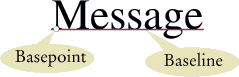
\includegraphics[height=0.1\paperheight,center]{pucrs-ep-fprog-unidade_04-lacos-laminas-message.png}
\end{figure}
	& \texttt{(x, y)} é o ponto base (\emph{basepoint}).\\
\hline
  \end{tabular}
\end{center}
}
\end{frame}

%-------------------------------------------------------
\begin{frame}[fragile]\frametitle{Gráficos em Java: alguns métodos de \texttt{Graphics} (3)}
{\scriptsize
\begin{center}
  \begin{tabular}{|p{6cm}|p{3cm}|p{4cm}|}
\hline
    \textbf{Método} & \textbf{Resultado} & \textbf{Explicação} \\
\hline
\texttt{g.setColor(color)}
&
A partir deste ponto, os métodos para desenhar ou desenhar preenchido usarão a cor selecionada.
& Use \texttt{Color.RED}, \texttt{Color.GREEN}, \texttt{Color.BLUE} e assim por diante.\\
\hline
  \end{tabular}
\end{center}
}
\end{frame}

%-------------------------------------------------------
\begin{frame}\frametitle{Gráficos em Java: exercícios}
\begin{enumerate}
	\item Escreva uma aplicação gráfica em Java para desenhar a seguinte face:
	\begin{figure}[h]
		
\includegraphics[height=2cm,center]{pucrs-ep-fprog-unidade_04-lacos-laminas-exercicio_1.png}
	\end{figure}
	{\tiny Fonte: Horstmann (2013, p. 197)}
	\item Escreva uma aplicação gráfica em Java para desenhar uma espiral retangular como a mostrada na figura a seguir:
	\begin{figure}[h]
		
\includegraphics[height=2cm,center]{pucrs-ep-fprog-unidade_04-lacos-laminas-exercicio_2.png}
	\end{figure}
	{\tiny Fonte: Horstmann (2013, p. 197)}
\end{enumerate}
\end{frame}

%=======================================================
\section{Referências}

%-------------------------------------------------------	
\begin{frame}\frametitle{Referências}
\noindent{HORSTMANN, C. \textbf{Java for Everyone – Late Objects}. 2. ed. Hoboken: Wiley, 2013. xxxiv, 589 p.}
\end{frame}

%=======================================================
\end{document}

